% Template for PLoS
% Version 3.4 January 2017
%
% % % % % % % % % % % % % % % % % % % % % %
%
% -- IMPORTANT NOTE
%
% This template contains comments intended 
% to minimize problems and delays during our production 
% process. Please follow the template instructions
% whenever possible.
%
% % % % % % % % % % % % % % % % % % % % % % % 
%
% Once your paper is accepted for publication, 
% PLEASE REMOVE ALL TRACKED CHANGES in this file 
% and leave only the final text of your manuscript. 
% PLOS recommends the use of latexdiff to track changes during review, as this will help to maintain a clean tex file.
% Visit https://www.ctan.org/pkg/latexdiff?lang=en for info or contact us at latex@plos.org.
%
%
% There are no restrictions on package use within the LaTeX files except that 
% no packages listed in the template may be deleted.
%
% Please do not include colors or graphics in the text.
%
% The manuscript LaTeX source should be contained within a single file (do not use \input, \externaldocument, or similar commands).
%
% % % % % % % % % % % % % % % % % % % % % % %
%
% -- FIGURES AND TABLES
%
% Please include tables/figure captions directly after the paragraph where they are first cited in the text.
%
% DO NOT INCLUDE GRAPHICS IN YOUR MANUSCRIPT
% - Figures should be uploaded separately from your manuscript file. 
% - Figures generated using LaTeX should be extracted and removed from the PDF before submission. 
% - Figures containing multiple panels/subfigures must be combined into one image file before submission.
% For figure citations, please use "Fig" instead of "Fig".
% See http://journals.plos.org/plosone/s/figures for PLOS figure guidelines.
%
% Tables should be cell-based and may not contain:
% - spacing/line breaks within cells to alter layout or alignment
% - do not nest tabular environments (no tabular environments within tabular environments)
% - no graphics or colored text (cell background color/shading OK)
% See http://journals.plos.org/plosone/s/tables for table guidelines.
%
% For tables that exceed the width of the text column, use the adjustwidth environment as illustrated in the example table in text below.
%
% % % % % % % % % % % % % % % % % % % % % % % %
%
% -- EQUATIONS, MATH SYMBOLS, SUBSCRIPTS, AND SUPERSCRIPTS
%
% IMPORTANT
% Below are a few tips to help format your equations and other special characters according to our specifications. For more tips to help reduce the possibility of formatting errors during conversion, please see our LaTeX guidelines at http://journals.plos.org/plosone/s/latex
%
% For inline equations, please be sure to include all portions of an equation in the math environment.  For example, x$^2$ is incorrect; this should be formatted as $x^2$ (or $\mathrm{x}^2$ if the romanized font is desired).
%
% Do not include text that is not math in the math environment. For example, CO2 should be written as CO\textsubscript{2} instead of CO$_2$.
%
% Please add line breaks to long display equations when possible in order to fit size of the column. 
%
% For inline equations, please do not include punctuation (commas, etc) within the math environment unless this is part of the equation.
%
% When adding superscript or subscripts outside of brackets/braces, please group using {}.  For example, change "[U(D,E,\gamma)]^2" to "{[U(D,E,\gamma)]}^2". 
%
% Do not use \cal for caligraphic font.  Instead, use \mathcal{}
%
% % % % % % % % % % % % % % % % % % % % % % % % 
%
% Please contact latex@plos.org with any questions.
%
% % % % % % % % % % % % % % % % % % % % % % % %

\documentclass[10pt,letterpaper]{article}
\usepackage[top=0.85in,left=2.75in,footskip=0.75in]{geometry}

\usepackage{float}

% amsmath and amssymb packages, useful for mathematical formulas and symbols
\usepackage{amsmath,amssymb}

% Use adjustwidth environment to exceed column width (see example table in text)
\usepackage{changepage}

% Use Unicode characters when possible
\usepackage[utf8x]{inputenc}

% textcomp package and marvosym package for additional characters
\usepackage{textcomp,marvosym}

% cite package, to clean up citations in the main text. Do not remove.
\usepackage{cite}

% Use nameref to cite supporting information files (see Supporting Information section for more info)
\usepackage{nameref,hyperref}

% line numbers
\usepackage[right]{lineno}

% ligatures disabled
\usepackage{microtype}
\DisableLigatures[f]{encoding = *, family = * }

% color can be used to apply background shading to table cells only
\usepackage[table]{xcolor}

% array package and thick rules for tables
\usepackage{array}

% Add links
\usepackage{hyperref}

% create "+" rule type for thick vertical lines
\newcolumntype{+}{!{\vrule width 2pt}}

% create \thickcline for thick horizontal lines of variable length
\newlength\savedwidth
\newcommand\thickcline[1]{%
  \noalign{\global\savedwidth\arrayrulewidth\global\arrayrulewidth 2pt}%
  \cline{#1}%
  \noalign{\vskip\arrayrulewidth}%
  \noalign{\global\arrayrulewidth\savedwidth}%
}

% \thickhline command for thick horizontal lines that span the table
\newcommand\thickhline{\noalign{\global\savedwidth\arrayrulewidth\global\arrayrulewidth 2pt}%
\hline
\noalign{\global\arrayrulewidth\savedwidth}}


% Remove comment for double spacing
%\usepackage{setspace} 
%\doublespacing

% Text layout
\raggedright
\setlength{\parindent}{0.5cm}
\textwidth 5.25in 
\textheight 8.75in

% Bold the 'Fig #' in the caption and separate it from the title/caption with a period
% Captions will be left justified
\usepackage[aboveskip=1pt,labelfont=bf,labelsep=period,justification=raggedright,singlelinecheck=off]{caption}
\renewcommand{\figurename}{Fig}

% Use the PLoS provided BiBTeX style
\bibliographystyle{plos2015}

% Remove brackets from numbering in List of References
\makeatletter
\renewcommand{\@biblabel}[1]{\quad#1.}
\makeatother

% Leave date blank
\date{}

% Header and Footer with logo
\usepackage{lastpage,fancyhdr,graphicx}
\usepackage{epstopdf}
\pagestyle{myheadings}
\pagestyle{fancy}
\fancyhf{}
\setlength{\headheight}{27.023pt}
\lhead{
\includegraphics[width=2.0in]{PLOS-submission.eps}}
\rfoot{\thepage/\pageref{LastPage}}
\renewcommand{\footrule}{\hrule height 2pt \vspace{2mm}}
\fancyheadoffset[L]{2.25in}
\fancyfootoffset[L]{2.25in}
\lfoot{\sf PLOS}


\begin{document}
\vspace*{0.2in}

% Title must be 250 characters or less.
\begin{flushleft}
{\Large
\textbf\newline{An interdisciplinary evaluation of community-based TURF-reserves} % Please use "sentence case" for title and headings (capitalize only the first word in a title (or heading), the first word in a subtitle (or subheading), and any proper nouns).
}
\newline
% Insert author names, affiliations and corresponding author email (do not include titles, positions, or degrees).
\\
Juan Carlos Villaseñor-Derbez\textsuperscript{1\Yinyang*},
Eréndira Aceves-Bueno\textsuperscript{1,2\Yinyang},
Stuart Fulton\textsuperscript{3\ddag},
Alvin Suarez\textsuperscript{3\ddag},
Arturo Hernández-Velasco\textsuperscript{3\ddag},
Jorge Torre\textsuperscript{3\ddag},
Fiorenza Micheli\textsuperscript{4\ddag}
\\
\bigskip
\textbf{1} Bren School of Environmental Science \& Management, University of California, Santa Barbara, Santa Barbara, CA, USA
\\
\textbf{2} Nicholas School of the Environment, Duke University, Beaufort, NC, USA
\\
\textbf{3} Comunidad y Biodiversidad A.C., Guaymas, Sonora, Mexico
\\
\textbf{4} Hopkins Marine Station and Stanford Center for Ocean Solutions, Stanford University, Pacific Grove, CA, USA
\\
\bigskip

% Insert additional author notes using the symbols described below. Insert symbol callouts after author names as necessary.
% 
% Remove or comment out the author notes below if they aren't used.
%
% Primary Equal Contribution Note
\Yinyang These authors contributed equally to this work.

% Additional Equal Contribution Note
% Also use this double-dagger symbol for special authorship notes, such as senior authorship.
\ddag These authors also contributed equally to this work.

% Current address notes
%\textcurrency Current Address: Dept/Program/Center, Institution Name, City, State, Country % change symbol to "\textcurrency a" if more than one current address note
% \textcurrency b Insert second current address 
% \textcurrency c Insert third current address

% Deceased author note
%\dag Deceased

% Group/Consortium Author Note
%\textpilcrow Membership list can be found in the Acknowledgments section.

% Use the asterisk to denote corresponding authorship and provide email address in note below.
* juancarlos@ucsb.edu

\end{flushleft}
% Please keep the abstract below 300 words
\section*{Abstract}
Coastal marine ecosystems provide livelihoods for small-scale fishers and coastal communities around the world. Small-scale fisheries face great challenges since they are difficult to monitor, enforce, and manage, which may lead to overexploitation. Combining territorial use rights for fisheries (TURF) with no-take marine reserves to create TURF-reserves can improve the performance of small-scale fisheries by buffering fisheries from environmental variability and management errors, while ensuring that fishers reap the benefits of conservation investments. Since 2012, 18 old and new community-based Mexican TURF-reserves gained legal recognition thanks to a regulation passed in 2012; their effectiveness has not been formally evaluated. We combine causal inference techniques and the Social-Ecological Systems framework to provide a holistic evaluation of community-based TURF-reserves in three coastal communities in Mexico. We find that, overall, reserves have not yet achieved their stated goals of increasing the density of lobster and other benthic invertebrates, nor increasing lobster catches. A lack of clear ecological and socioeconomic effects likely results from a combination of factors. First, some of these reserves might be too young for the effects to show (reserves were 6 - 10  years old). Second, the reserves are not large enough to protect mobile species, like lobster. Third, variable and extreme oceanographic conditions have impacted harvested populations. Fourth, local fisheries are already well managed, and while reserves may protect populations within its boundaries, it is unlikely that reserves might have a detectable effect in catches. However, even small reserves are expected to provide benefits for sedentary invertebrates over longer time frames, with continued protection. These reserves may provide a foundation for establishing additional, larger marine reserves needed to effectively conserve mobile species.

% Please keep the Author Summary between 150 and 200 words
% Use first person. PLOS ONE authors please skip this step. 
% Author Summary not valid for PLOS ONE submissions.   
%\section*{Author summary}
%Lorem ipsum dolor sit amet, consectetur adipiscing elit. Curabitur eget porta erat. Morbi consectetur est vel gravida pretium. Suspendisse ut dui eu ante cursus gravida non sed sem. Nullam sapien tellus, commodo id velit id, eleifend volutpat quam. Phasellus mauris velit, dapibus finibus elementum vel, pulvinar non tellus. Nunc pellentesque pretium diam, quis maximus dolor faucibus id. Nunc convallis sodales ante, ut ullamcorper est egestas vitae. Nam sit amet enim ultrices, ultrices elit pulvinar, volutpat risus.

\clearpage

\linenumbers

% Use "Eq" instead of "Equation" for equation citations.
\section*{Introduction}

Marine ecosystems around the world sustain significant impacts due to overfishing and unsustainable fishing practices \cite{pauly_2005-qV,worm_2006-IB,halpern_2008-dK}. In particular, small-scale fisheries face great challenges since they tend to be hard to monitor and enforce, given the large number of participants, heterogeneity in fleet, gears, and targeted species; as well as seasonality and geographical distribution \cite{costello_2012,jacquet_2008}. One of the many approaches taken to improve the performance of coastal fisheries and health of the local resources is through the implementation of Territorial Use Rights for Fisheries (TURFs) that contain no-take marine reserves \cite{afflerbach_2014,gelcich_2015,lester_2017}.

TURFs are a fisheries management tool in which a well-defined group of fishers (\emph{e.g.} fishing cooperatives) have exclusive access to an explicitly delimited portion of the ocean. They promote a sense of stewardship and incentivise resource users to sustainably manage their resources \cite{gelcich_2008,costello_2010,mccay_2014}. On the other hand, no-take marine reserves (marine reserves from hereinafter) are areas where all extractive activities are off-limits. These can be implemented to protect biodiversity but also as fishery management tools to aid in the recovery of marine stocks. These instruments can be combined by establishing a marine reserve within a TURF, thus making them TURF-reserves \cite{afflerbach_2014,gelcich_2015,lester_2017}.

Conservation science has shown how well implemented and enforced marine reserves may lead to increased biomass, species richness, and abundance within the protected regions \cite{halpern_2002,lester_2009}, and that these may have a series of additional benefits such as mitigation and adaptation to climate change effects, protection from environmental variability, and fisheries benefits \cite{roberts_2017-J9,micheli_2012-EU,krueck_2017-J1}. Likewise, research on TURFs has shown that these areas have higher abundance of targeted species than sites operating under open access and even similar to that of marine reserves \cite{gelcich_2008,gelcich_2012}. The benefits resulting from reserves established within TURFs (\emph{i.e.} TURF-reserves) should be captured exclusively by the group of fishers with exclusive access \cite{gelcich_2015}. Although in theory these systems are expected to be successful \cite{smallhornwest_2018}, there is little empirical evidence of their effectiveness and the drivers of their success.

Recent changes in fisheries regulation in Mexico provide a ripe opportunity to study the effectiveness of community-based TURF-reserves in small-scale fisheries. In Mexico, a legal framework created in 2012 allows fishers to request legal recognition of community-based reserves as “Fish Refuges” (\emph{Zona de Refugio Pesquero}, described in more detail below; \cite{nom}). Since 2012, 45 old and new marine reserves have gained legal recognition as Fish Refuges. Of these, 18 were originally implemented within TURFs. However, their effectiveness has not yet been reported in the scientific literature.

Marine reserves have largely been evaluated from an ecological perspective, focusing on ecological indicators such as biomass and species richness or spillover\cite{halpern_2002,lester_2009,krueck_2017-J1}. However, TURF-reserves are intricate social-ecological systems, often implemented with a combination of ecological and social objectives. A customary evaluation of TURF-reserves is unlikely to provide an accurate representation of the changes, benefits, and limitations of such an intervention.

The objective of this work is twofold. First, to provide a holistic evaluation of the effectiveness of community-based TURF-reserves in terms of the changes in biological and socioeconomic indicators and the governance settings under which these develop, which may inform similar processes in other countries. The second objective is to identify opportunities where improvement or adjustment might lead to increased effectiveness of these reserves. We combine causal inference techniques and the Social-Ecological Systems (SES) framework to evaluate community-based TURF-reserves in three coastal communities in Mexico.  Our work highlights the benefits of taking an interdisciplinary approach to marine reserve evaluation, and provides a robust evaluation of TURF-reserve effectiveness that may inform adaptive management and future interventions.

\section*{Methods}

\subsection*{TURF-reserves in Mexico}

Community-based marine reserves that are implemented within TURFs are a form of TURF-reserve, voluntarily established and enforced by local communities. Community-based spatial closures occur elsewhere, like the \emph{kapu} or \emph{ra’ui} areas in the Pacific Islands \cite{johannes_2002,bohnsack_2004}. This bottom-up approach can increase compliance and self-enforcement, and reserves can yield benefits similar to systematically-designed reserves \cite{beger_2004,smallhornwest_2018}. However, community-based reserves can be hard to enforce if they are not legally recognized. In such conditions, TURF fishers must rely on the exclusive access of the TURF to maintain high levels of compliance.

In an effort to bridge this normative gap, Mexican Civil Society Organizations (CSOs) served as a link between fishers and government, and helped create a legal framework that solves this governance issue: Fish Refuges \cite{nom}. Fish Refuges can be implemented as permanent, temporary or partial reserves, which can protect one, some, or all resources within their boundaries. One of the ways in which fishing communities have taken advantage of this new tool is by implementing temporary marine reserves within their TURFs with a defined expiration date (often five years). When the expiration date is reached, fishers can chose to open the reserves to fishing or re-establish them. Our work focuses on Fish Refuges implemented as community-based TURF-reserves in small-scale fisheries.

The most common setup of community-based TURF-reserves in Mexico is the following. Fishers from a given community assemble into a fishing cooperative which has exclusive fishing rights over a spatially delimited area (\emph{i.e.} TURFs shown as blue polygons in Fig~\ref{fig:map}A). Each TURF is exclusively fished by one cooperative, and each community usually hosts no more than one cooperative. The profits from each TURF are shared amongst all fishers from the cooperative \cite{mccay_2014,mccay_2017}. Fishing cooperatives interested in implementing marine reserves within their TURFs (\emph{i.e.} TURF-reserves) work with CSOs to design them. Fishers then ask the government to grant legal recognition to their TURF-reserves as Fish Refuges, as stated in the 2014 regulation \cite{nom}.

\begin{figure}[!h]
\centering
%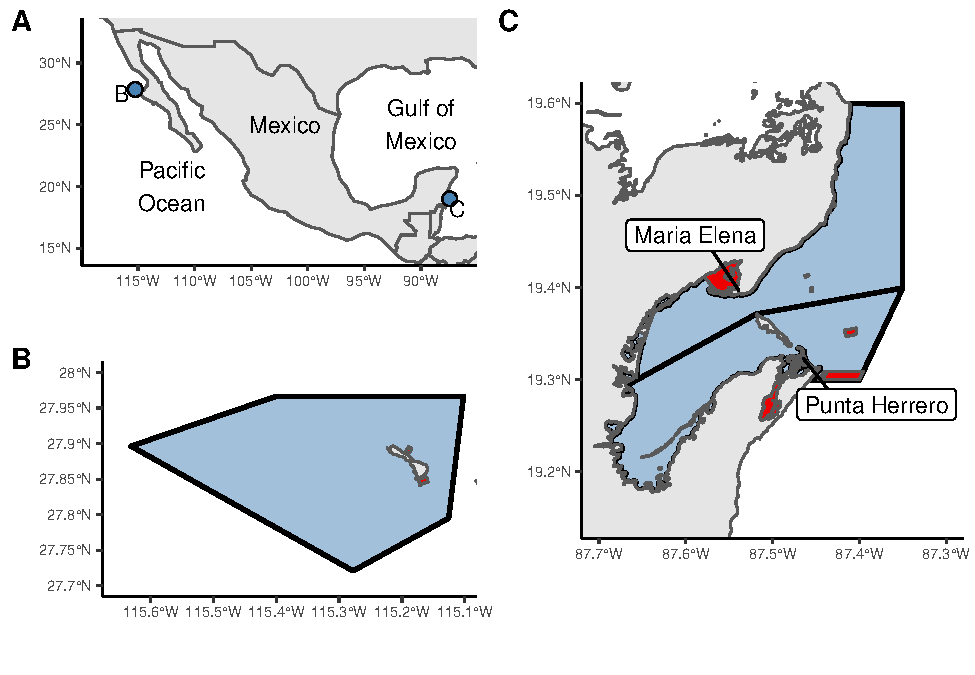
\includegraphics{img/fig_map.pdf}
\caption{Location of the three coastal communities studied (A). Isla Natividad (B) is located off the Baja California Peninsula, Maria Elena and Punta Herrero (C) are located in the Yucatan Peninsula. Blue polygons represent the TURFs, and red polygons the marine reserves.}
\label{fig:map}
\end{figure}

\subsection*{Study areas}

We evaluate three community-based no-take TURF-reserve systems implemented in Mexican TURF-managed fisheries (Fig~\ref{fig:map}A). The first one was created by the \emph{Buzos y Pescadores de la Baja California} fishing cooperative, located in Isla Natividad in the Baja California Peninsula (Fig~\ref{fig:map}B). At present, the main fishery in the island is the spiny lobster (\emph{Panulirus interruptus}), but other resources like finfish, sea cucumber, sea urchin, snail, and abalone are also an important source of income. In 2006, the community decided to implement two marine reserves within their fishing grounds. The objective of these reserves was "to protect and recover stocks of commercially important invertebrate species"; mainly lobster and abalone. The reserves were implemented and enforced by the community since 2006, but obtained legal recognition in 2018 \cite{dof_website_2018}.

The other two TURF-reserve systems are located in Maria Elena and Punta Herrero, in the Yucatan Peninsula (Fig~\ref{fig:map}C). In contrast with Isla Nativdad, which hosts a well-established fishing community, Maria Elena is a fishing camp visited intermittently during the fishing season that belongs to the \emph{Cozumel} fishing cooperative. Punta Herrero is home to the \emph{José María Azcorra} fishing cooperative, and similar to Isla Natividad hosts a small community. Their main fishery is the Caribbean spiny lobster (\emph{Panulirus argus}), but they also target finfish in the off-season. Maria Elena and Punta Herrero established eight and four marine reserves in 2012 and 2013, respectively. These reserves have been legally recognized as Fishing Refuges since their original implementation \cite{dof_website_2012,dof_website_2013} and subsequent re-establishments in 2017 \cite{dof_website_2017b}.

These communities are representative of their region in terms of ecology, socioeconomic, and governance aspects. Isla Natividad, for example, is part of a greater group of fishing cooperatives belonging to a Federation of Fishing Cooperatives. This group has been identified as a cohesive group that cooperates to better manage their resources \cite{mccay_2014,mccay_2017,acevesbueno_2017}. Likewise, Maria Elena and Punta Herrero are representative of fishing cooperatives in the Mexican Caribbean, which are also part of a regional Federation. Together, these three communities provide an accurate representation of other fishing communities that have been historically managed with TURFs in each of their regions. While each region has additional communities that have established community-based TURF-reserves, available data would not allow us to perform the in-depth causal inference analysis that we undertake. Yet, given the similarities among communities and the socioeconomic and governance setting under which they operate, it is safe to cautiously generalize our insights to other similar community-based TURF-reserves in Mexico and elsewhere.

The regulation governing the implementation of Fish Refuges states that these are fishery management tools intended to have conservation and fisheries benefits \cite{nom}. For this reason, the main portion of our analyses focuses on a series of biological and socioeconomic indicators that may respond to reserve implementation. However, the effectiveness of conservation and fisheries management interventions also depends on the social and governance structures in place. We therefore incorporate a reduced version of the Social Ecological Systems framework \cite{ostrom_2009} and evaluate variables and indicators known to aid and hinder the effectiveness of management interventions in conservation and fisheries. The incorporation of the SES is not intended to relate different levels of governance with reserve effectiveness, but rather to provide context on the social-ecological system in which reserves develop. The following two sections describe our data collection methods and analyses.

\subsection*{Data collection}

We use three main sources of information to evaluate these reserves across ecological, socioeconomic, and governance dimensions. Biological data come from the annual ecological monitoring of reserve and control sites. Reserve sites are areas where no fishing occurs. Control sites are areas that meet the following criteria: i) habitat characteristics are similar to the corresponding reserves, ii) presumably had a similar probability of being selected as reserves during the design phase, iii) are located within the TURF, where fishing occurs, and iv) are not directly adjacent to the reserves to avoid confounding due to spillover effect (sites were at least 1 km apart). We focus our evaluation on sites where data are available for reserve and control sites, before and after the implementation of the reserve. This provides us with a Before-After-Control-Impact (\emph{i.e.} BACI) sampling design that allows us to capture and control for temporal and spatial dynamics and causally attribute the changes to the reserve \cite{stewartoaten_1986,francinifilho_2008,depalma_2018,kerr_2019,Villasenor-Derbez_2018}.

The biological data are collected by members from each community and personnel from the Mexican CSO \emph{Comunidad y Biodiversidad} (\href{https://www.cobi.org.mx}{COBI}). Trained divers record species richness and abundances of fish and invertebrate species along replicate transects (30 $\times$ 2 m each) at depths 5-20 m in the reserves and control sites \cite{suman_2010-ez,fulton_2018,fulton_2019}. Size structures are also collected during fish surveys, where divers estimate fish length to the nearest centimeter. All sites were surveyed annually, and at least once before implementation of the reserves. A summary of sampling effort and time series, as well as species checklist, are shown in the supplementary materials (Tables A-B, Figures A-D, and Tables I-J in \nameref{S1_Text}).

Socioeconomic data contain monthly lobster landings (Kg) and revenues (in Mexican Pesos; MXP) for TURF-managed cooperatives with and without marine reserves. These were requested from the National Commission for Aquaculture and Fisheries (\emph{Comisión Nacional de Acuacultura y Pesca}; CONAPESCA) via the access to information act. In this case our treated unit are the cooperatives (\emph{i.e.} communities) that have implemented a reserve within their TURF, and the controls are adjacent communities that have a TURF but did not implement a reserve. Cooperatives incorporated in this analysis have similar number of members, belong to larger regional-level Cooperative Federations, and are exposed to the same markets and institutional frameworks, making them plausible controls \cite{mccay_2014,mccay_2017,ayer_2018}. Landings and revenues were aggregated at the cooperative-year level, and revenues were adjusted to represent 2014 values by the Consumer Price Index for Mexico \cite{oecd_2017}. A table with summary statistics and time series for this data are provided in the supplementary materials (Table C and Figure E in \nameref{S1_Text}).

Data for the evaluation of the SES were collected at the community-level, and focused on the Resource Systems, Resource Units, Actors, and Governance System (Table~\ref{table:ses}). Data come from official documents used in the design, creation, and implementation of the marine reserves. These include the technical studies that the cooperatives submit when they request recognition of their reserves, as well as the official enactments \cite{dof_website_2012,dof_website_2013,dof_website_2018}. We also complimented information based on the authors' experience and knowledge of the communities (RS5, RU5, A3, GS6.2, GS99.1, GS9.2, and GS10.1). In Table~\ref{table:ses}, the alphanumeric codes follow \cite{basurto_2013-oq}, and an asterisk denotes variables incorporated based on \cite{difranco_2016-Xw} and \cite{edgar_2014-UO}.

\begin{table}[!ht]

\caption{{\bf Variables for the Social-Ecological System analysis.}}
\centering
\resizebox{\linewidth}{!}{
\begin{tabular}{>{\raggedright\arraybackslash}p{6.5cm}|>{\raggedright\arraybackslash}p{12.2cm}}
\hline
Variable & Narrative\\
\hline
\multicolumn{2}{l}{\textbf{Resource System (RS)}}\\
\hline
\hspace{1em}RS2 - Clarity of system boundaries: Clarity of geographical boundaries of TURF and reserves & Individual TURF and reserve boundaries are explicitly outlined in official documents that include maps and coordinates. Reserve placement is decided by the community. Fishers use GPS units and landmarks.\\
\hline
\hspace{1em}RS3 - Size of resource system: TURF Area (Km$^2$) & IN = 889.5; ME = 353.1; PH = 299.7\\
\hline
\hspace{1em}RS3 - Size of resource system: Reserve area (Evaluated reserve area; Km$^2$) & IN = 2 (1.3); ME = 10.48(0.09); PH = 11.25 (4.37)\\
\hline
\hspace{1em}RS4.1 - Stock status: Status of the main fishery & Lobster stocks are well managed, and are (IN) or have been (ME, PH) certified by the Marine Stewardship Council.\\
\hline
\hspace{1em}*RS5 - Age of reserves: Years since reserves were implemented & IN = 12; ME = 6; PH = 5\\
\hline
\multicolumn{2}{l}{\textbf{Resource Unit (RU)}}\\
\hline
\hspace{1em}RU1 - Resource unit mobility & Adult spiny lobsters can move between 1 and 10 Km, while larvae can have displacements in the order of hundreds of Km (Aceves-Bueno et al., 2017; Green et al., 2017).\\
\hline
\hspace{1em}RU5 - Number of units (catch diversity): Number of targeted species & Lobster is their main fishery of these three communities, but they also target finfish (2 spp each). Additionally, fishers from Isla Natividad target other sedentary benthic invertebrates (4 spp).\\
\hline
\multicolumn{2}{l}{\textbf{Actors (A)}}\\
\hline
\hspace{1em}A1 - Number of relevant actors: Number of fishers & IN = 98; ME = 80; PH = 21\\
\hline
\hspace{1em}*A3 - Isolation: Level of isolation of the fishing grounds & Their fishing grounds and reserves are highly isolated and away from dense urban centers. IN lies 545 Km south from Tijuana, and ME and PH 230 Km south from Cancun, where the nearest international airports are located.\\
\hline
\multicolumn{2}{l}{\textbf{Governance system (G)}}\\
\hline
\hspace{1em}GS6.1.4.3 - Territorial use communal rights : Presence of institutions that grant exclusive harvesting rights & Each community has exclusive access to harvest benthic resources, including lobster. These take the form of Territorial User Rights for Fisheries granted by the government to fishing cooperatives.\\
\hline
\hspace{1em}GS6.2 - Operational rules: Rules implemented by individuals atuhorized to partake on collective activities & Fishers have rules in addition to what the legislation mandates. These are: larger minimum catch sizes, lower quotas, and assigning fishers to specific fishing grounds within their TURF.\\
\hline
\hspace{1em}GS9.1 - Social monitoring: Monitoring of the activities performed by cooperative members and external fishers & Fishing cooperatives have a group (Consejo de vigilancia) that monitors and enforces formal and internal rules. They ensure fishers of their fishing cooperative adhere to the established rules, and that foreign vessels do not poach their TURF and reserves.\\
\hline
\hspace{1em}GS9.2 - Biophysical monitoring: Monitoring of biological resources, including targeted species & Fishers perform annual standardized underwater surveys in the reserves and fishing grounds. Recently, they have installed oceanographic sensors to monitor oceanographic variables.\\
\hline
GS10.1 - Graduated sanctions & Fishers have penalties for breaking collective-choice rules or fishing inside the reserves. These may range from scoldings and warnings to not being allowed to harvest a particular resource or being expelled from the cooperative.\\
\hline
\end{tabular}}
\label{table:ses}
IN = Isla Natividad, ME = Maria Elena, PH = Punta Herrero. The presented narrative applies equally for all communities unless otherwise noted. An asterisk (*) denotes variables incorporated into the framework.
\end{table}

\clearpage

\subsection*{Data analysis}

We evaluate the effect that the TURF-reserves have had on four ecological and two socioeconomic indicators shown in Table~\ref{table:indicators}. Recall that reserves were implemented to protect lobster and other benthic invertebrates. However, we also use the available fish and invertebrate data to test for associated co-benefits.

\begin{table}[!ht]

\caption{
{\bf List of indicators used to evaluate the effectiveness of marine reserves, grouped by category.}}
\centering
\begin{tabular}{l|l}
\hline
Indicator & Units\\
\hline
\multicolumn{2}{l}{\textbf{Biological}}\\
\hline
\hspace{1em}Lobster density & org $\mathrm{m}^{-2}$\\
\hline
\hspace{1em}Invertebrate density & org $\mathrm{m}^{-2}$\\
\hline
\hspace{1em}Fish density & org $\mathrm{m}^{-2}$\\
\hline
\hspace{1em}Fish biomass & Kg $\mathrm{m}^{-2}$\\
\hline
\multicolumn{2}{l}{\textbf{Socioeconomic}}\\
\hline
\hspace{1em}Income from target species & M MXP\\
\hline
\hspace{1em}Landings from target species & Metric Tonnes\\
\hline
\end{tabular}
\label{table:indicators}
\end{table}

We use a difference-in-differences analysis to evaluate these indicators. This approach is widely used in econometric literature to estimate the average treatment effect of an intervention, like the impact of minimum wage increases on employment rates \cite{card_1994}. In our case it allows us to estimate the effect that the reserve had on each biological and socioeconomic indicator (Table~\ref{table:indicators}) by comparing trends across time and treatments since reserve implementation \cite{moland_2013,Villasenor-Derbez_2018, kerr_2019}. To perform difference-in-differences, we regress the indicator of interest on a dummy variable for treatment, a dummy variable for years, and the interaction term between these with a multiple linear regression of the form:

\begin{equation}
I_{i,t} = \alpha + \gamma_{t} Year_t + \beta Zone_i + \lambda_{t} Year_t\times Zone_i + \epsilon_{i,t}
\label{eqn:reg_bio}
\end{equation}

Where year-level fixed effects capturing a temporal trend are represented by $\gamma_t Year_t$, and $\beta Zone_i$ captures the difference between reserve ($Zone = 1$) and control ($Zone = 0$) sites. The effect of the reserve is captured by the $\lambda_t$ vector of coefficients, and represents the difference observed between the control site before the implementation of the reserve and the treated sites at time $t$ after controlling for other time and space variations (\emph{i.e.} $\gamma_t$ and $\beta$ respectively). Therefore, we would expect this term to be positive if the indicator increases because of the reserve. Finally, $\epsilon_{i,t}$ represents the error term of the regression.

Socioeconomic indicators are evaluated with a similar approach. Due to data constrains, we only evaluate socioeconomic data for Isla Natividad (2000 - 2014) and Maria Elena (2006 - 2013). Neighboring communities are used as counterfactuals that allow us to control for unobserved time-invariants. Each focal community (\emph{i.e.} Isla Natividad and Maria Elena) has three counterfactual communities.

\begin{equation}
I_{i,t} = \alpha + \gamma_{t} Year_t + \beta Treated_i + \lambda_{t} Year_t\times Treated_i +\epsilon_{i,t}
\label{eqn:soc_reg}
\end{equation}

The coefficient interpretations remains as for Eq. \ref{eqn:reg_bio}, but in this case the $Treated$ dummy variable indicates if the community has a reserve ($Treated = 1$) or not ($Treated = 0$).

These regression models allow us to establish a causal link between the implementation of marine reserves and the observed trends by accounting for temporal and site-specific dynamics \cite{depalma_2018}. Since we are interested in the effectiveness of each reserve system, we fit one model for each indicator in each community (\emph{e.g.} there are three models for lobster density, one for each community). This gives us a total of 12 biological model fits and four socioeconomic model fits. Model coefficients were estimated via ordinary least-squares and used heteroskedastic-robust standard error correction \cite{zeileis_2004-7n}. All analyses were performed in R 3.5.2 and R Studio version 1.1.456 \cite{R_2018}. All data and code needed to reproduce our analyses are available in a GitHub repository at: \url{https://github.com/jcvdav/ReserveEffect}.

TURF-reserve systems are inherently intricate social-ecological systems, and their effectiveness must depend on how environmental and social factors combine and interact \cite{ostrom_2009,gelcich_2015}. When evaluating the effects of TURF-reserves, it is important to consider not only the indicators of interest, but also the governance settings under which a reserve operates. We use the SES framework to qualitatively evaluate each community and create a narrative that provides context for each of them. The use of this framework standardizes our analysis and allows us to communicate our results in a common language across fields by using a set of previously defined variables and indicators. Due to the lack of sufficient information to quantitatively operationalize the social-ecological systems framework for these case studies (as done in \cite{leslie_2015-na}), we followed a similar approach to \cite{basurto_2013-oq}, who used the SES framework as a classification system of the available information to qualitatively analyze fisheries systems. We based our variable selection primarily on previous analyses of Mexican fishing cooperatives \cite{leslie_2015-na,basurto_2013-oq}. We also incorporate other relevant variables known to influence reserve performance, such as age and size of reserve or isolation of the system \cite{difranco_2016-Xw,edgar_2014-UO}. Table~\ref{table:ses} shows the selected variables, along with definitions and values.

\section*{Results}

The following sections present the effect that marine reserves had on the biological and socioeconomic indicators for each coastal community. Results are presented in terms of difference through time and across sites, relative to the control site on the year of implementation (\emph{i.e.} the difference-in-differences estimate or effect size $\lambda_t$ from Eqs. \ref{eqn:reg_bio} and \ref{eqn:soc_reg}). We also provide an overview of the governance settings of each community, and discuss how these might be related to the effectiveness and performance of the reserves.

\subsection*{Biological effects}

Indicators showed ambiguous responses through time for each reserve. Fig~\ref{fig:indicators}A shows positive effect sizes for lobster densities in Isla Natividad and Punta Herrero during the first years, but the effect is eroded through time. In the case of Maria Elena, positive changes were observed in the second and third years. These effects were in the order of 0.01 extra organisms $\mathrm{m}^{-2}$, but were only significantly different from zero for Maria Elena ($p < 0.05$). Likewise, no significant changes were detected in fish biomass or invertebrate and fish densities (Fig. \ref{fig:indicators}B-D). Invertebrate and fish densities showed positive trends in all reserves for some years. However, these were not statistically significant. Figures with time series of indicators and tables with model coefficients and main effects are presented in the supplementary materials (Figures A-D and Tables D-F in \nameref{S1_Text}).

\begin{figure}[h]
\centering
%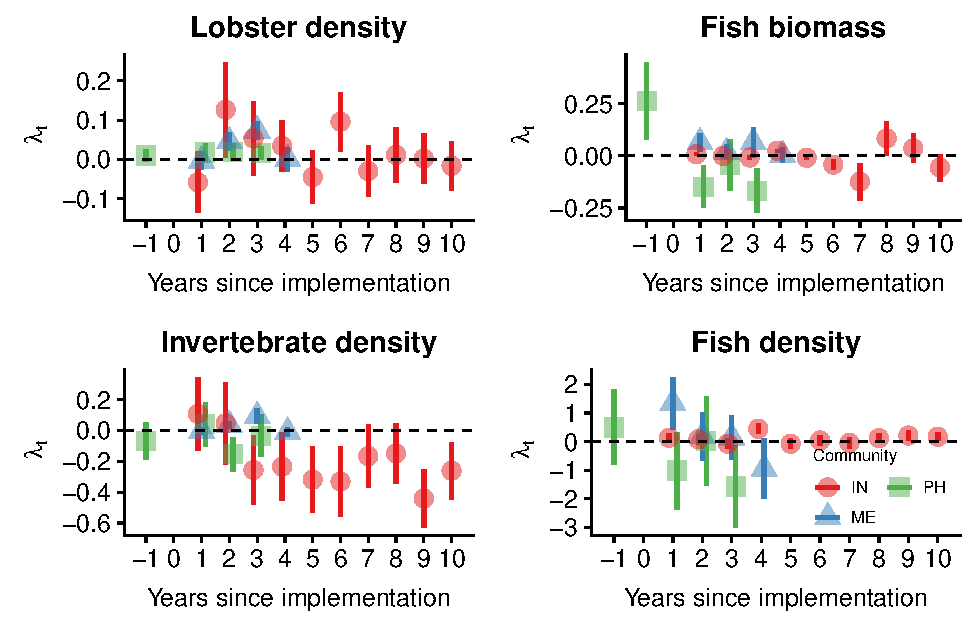
\includegraphics{img/fig_bio_results.pdf}
\caption{{\bf Effect sizes for biological indicators}
Points indicate the effect size and error bars are heteroskedastic-robust standard errors. Years have been centered to year of implementation. Colors and shapes denote communities: Isla Natividad (IN; red circles), Maria Elena (ME; blue triangles), and Punta Herrero (PH; green squares). Points are jittered hotizontally to avoid overplotting.}
\label{fig:indicators}
\end{figure}

\subsection*{Socioeconomic effects}

Lobster landings and revenue were only available for Isla Natividad and Maria Elena (Fig~\ref{fig:lobsters}). For all years before implementation, the effect sizes are close to zero, indicating that the control and treatment sites have similar pre-treatment trends, suggesting that these are plausible controls. However, effect sizes do not change after the implementation of the reserve. Interestingly, the negative effect observed for Isla Natividad on year 5 corresponds to the 2011 hypoxia events \cite{micheli_2012-EU}. The only positive change observed in lobster landings is for Isla Natividad in 2014 ($p < 0.1$). The year of post-implementation data for Maria Elena does not show a significant effect of the reserve. Isla Natividad shows higher revenues after the implementation of the reserve, as compared to the control communities, though these changes are only significant for the third year ($p < 0.05$). Full tables with model coefficients are presented in the supplementary materials (Tables G-H in \nameref{S1_Text}).

\begin{figure}[!h]
\centering
%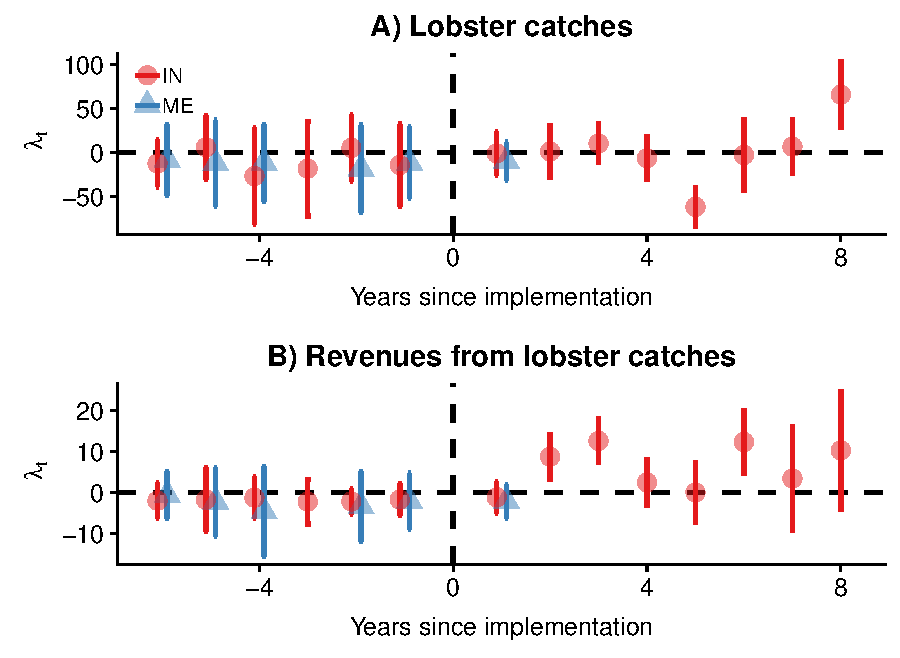
\includegraphics{img/fig_socioeco_results.pdf}
\caption{{\bf Effect sizes for socioeconomic indicators}
Points indicate the effect size and error bars are heteroskedastic-robust standard errors for lobster catches and revenues at Isla Natividad (IN; red circles) and Maria Elena (ME; blue triangles). Years have been centered to year of implementation. Points are jittered hotizontally to avoid overplotting.}
\label{fig:lobsters}
\end{figure}

\subsection*{Governance}

We find that the analyzed communities share similarities known to foster sustainable resource management and increase reserve effectiveness. For example, fishers operate within clearly outlined TURFs (RS2, GS6.1.4.3) that provide exclusive access to resources and reserves. Along with their relatively small groups (A1 - Number of relevant actors), Isolation (A3), Operational rules (GS6.2), Social monitoring (GS9.1), and Graduated sanctions (GS10.1), these fisheries have strong governance structures that enable them to monitor their resources and enforce rules to ensure sustainable management \cite{mccay_2014,ayer_2018}.

In general, success of conservation initiatives depends on the incentives of local communities to maintain a healthy status of the resources upon which they depend \cite{jupiter_2017}. Due to the clarity of access rights and isolation, the benefits of conservation directly benefit the members of the fishing cooperatives, which have favored the development of efficient community-based enforcement systems. However, our SES analysis also highlights factors that might hinder reserve performance or mask outcomes. While total reserve size ranges from 0.2\% to 3.7\% of the TURF area, individual reserves are often small (RS3); the largest reserve is only 4.37 km\textsuperscript{2}, and the smallest one is 0.09 km\textsuperscript{2}. Reserves are also relatively young (RS5). Additionally, fishers harvest healthy stocks (RS4.1), and it is unlikely that marine reserves will result in increased catches.

\section*{Discussion}

Our results indicate that these TURF-reserves have not increased lobster densities. Additionally, no co-benefits were identified when using other ecological indicators aside from the previously reported buffering effect that reserves can have to environmental variability in Isla Natividad, as well as positive trends in invertebrate and fish densities \cite{micheli_2012-EU,Villasenor-Derbez_2018}. The socioeconomic indicators pertaining landings and revenues showed little to no change after reserve implementation. Our qualitative implementation of the social-ecological systems framework allowed us to systematically identify important differences between the case studies’ governance systems and incorporate other characteristics of these fisheries neglected during the process of data collection (Table~\ref{table:ses}). These communities exhibit all the social enabling conditions for effective reserve and resource management. Here we discuss possible shortcomings in our analyses as well possible explanations for the lack of effectiveness.

While many ecology studies have used BACI sampling designs and respective analyses (\emph{e.g.} \cite{stewartoaten_1986}), few conservation studies have done so to evaluate the effect of an intervention (\emph{e.g.} \cite{francinifilho_2008,lester_2009,moland_2013,kerr_2019}) which has resulted in a call for more robust analyses in conservation science \cite{guidetti_2002,ferraro_2006}. Our approach to evaluate the temporal and spatial changes provides a more robust measure of reserve effectiveness, and captures previously described patterns. For example, the rapid increase observed for lobster densities in Isla Natividad on the sixth year (\emph{i.e.} 2012; Fig. \ref{fig:indicators}A), occurs a year after the hypoxia events described by \cite{micheli_2012-EU}, which caused mass mortality of sedentary organisms such as abalone and sea urchins, but not lobster and finfish.

While the use of causal inference techniques may help us support evidence-based conservation, spatial connectivity between reserve and control sites, stockpiling, and backstopping may confound the results \cite{kerr_2019}. Given that we find no clear evidence of reserve effectiveness, one might say that our reserve and control sites are not spatially independent. This would imply that the recovery within the reserve quickly results in recovery outside the protected area. However, indicators show little to no temporal variation (Figures A-D in \nameref{S1_Text}), and it is unlikely that this effect would be observed under current reserve designs, as detailed below.

Our analyses of socioeconomic indicators has three limitations. First, we only look at landings and revenues by landings for communities with and without TURF-reserves. There are a number of other possible indicators that could show a change due to the implementation of the reserve. Notably, one often cited in the literature is additional benefits, such as tourism \cite{viana_2017}. However, it is unlikely that the evaluated communities will experience tourism benefits due to their remoteness and the lack of proper infrastructure to sustain tourism. A second limitation of our socioeconomic analysis is that we do not observe effort data, which may mask the effect of the reserve. For example, if catches remain relatively unchanged but fishing effort decreased, that would imply a larger catch per unit effort and thus higher profitability, provided that cost per unit effort does not increase. Likewise, it is possible that fishing effort increased around reserves to maintain the historical levels of landings. A final limitation applies to Maria Elena, where we only observe landings and income for one year after reserve implementation. While one would not expect to observe increased landings or income in such a short period, a spatial closure might cause total catches to decline, especially if effort is held constant.

Lack of evidence of reserve effectiveness is commonly associated to lack of proper enforcement and compliance, as well as capacity shortfalls \cite{edgar_2014-UO,difranco_2016-Xw,gill_2017}. However, it is unlikely that the evaluated reserves are subject to these common problems. The reserves are implemented within TURFs, which provide a sense of ownership of resources and promotes sustainable management \cite{mccay_2017}. The same incentives that ensure sustainable management in a TURF should extend to the reserves that these contain. This is supported by our SES analysis, which suggests that these communities exhibit strong governance and enforcement structures. Instead, the lack of effectiveness observed may be driven by a combination of factors, such as age of the reserves, sub-optimal reserve design, or environmental variation. The next paragraphs provide a detailed discussion of these possible causes.

A first possible explanation for the lack of effectiveness may be the young age of the reserves. Literature shows that age and enforcement are important factors that influence reserve effectiveness \cite{edgar_2014-UO,babcock_2010}. Isla Natividad has the oldest reserves, and our SES analysis suggests that all communities have a well-established community-based enforcement system. With these characteristics, one would expect the reserves to be effective. In fact, the oldest reserves show some positive trends for invertebrate and fish densities, as well as income. Maria Elena and Punta Herrero are relatively young reserves (\emph{i.e.} \textless 6 years old; RS5 in Table~\ref{table:ses}) and effects may not yet be evident; community-based marine reserves in tropical ecosystems may take six years or more to show a spillover effect \cite{dasilva_2015-zX}. 

Another key condition for effectiveness is reserve size \cite{edgar_2014-UO}, and the lack of effectiveness can perhaps be attributed to poor ecological coherence in reserve design (\emph{sensu} \cite{rees_2018}). In Isla Natividad, the reserves can yield fishery benefits for the abalone fishery \cite{rossetto_2015-V0}, however, abalone are less mobile than lobsters, and perhaps the reserves provide enough protection to these sedentary molusks, but not lobsters. Small reserves in the Mediterranean Sea have shown that the effect of a reserve is only observable for species with a home range smaller than the reserve \cite{difranco_2018}. However, design principles developed for marine reserves in the Caribbean state that reserves "should be more than twice the size of the home range of adults and juveniles", and suggest that reserves seeking to protect spiny lobsters should have at least 14 km across \cite{green_2017}. As shown in the SES analysis, the size of the marine reserves appears small compared to the movement capacity of the main targeted species (RU1, RS3; Table~\ref{table:ses}). Furthermore, fishers may favor implementation of reserves that pose low fishing costs due to their small size or location. Our analysis of economic data supports this hypothesis, as neither landings nor revenues showed the expected short-term reductions associated to the first years of reserve implementation \cite{ovando_2016-Wg}.

Even if reserves had appropriate sizes and were placed in optimal locations, there are other plausible explanations for the observed patterns. For instance, marine reserves are only likely to provide fisheries benefits if initial population sizes are low and the fishery is poorly managed \cite{hilborn_2004,hilborn_2006}. Both lobster fisheries were certified by the Marine Stewardship Council and are managed via species-specific minimum catch sizes, seasonal closures, protection of "berried" females, and escapement windows where traps are allowed \cite{dof_website_1993}. It is uncertain whether such a well-managed fishery will experience additional benefits from small marine reserves; reserves implemented in TURFs where fishing pressure is already optimally managed will still show a trade-off between fisheries and conservation objectives \cite{lester_2017}. In contrast, invertebrate fisheries have seen declining catches and finfish fisheries are not managed under TURFs, which may explain the positive trends observed. Furthermore, TURFs alone can have greater biomass and richness than areas operating under open access \cite{gelcich_2008}. This might reduce the difference between indicators from the TURF and reserve sites, making it difficult to detect such a small change. Further research should focus on evaluating sites in the reserve, TURF, and open access areas or similar Fish Refuges established without the presence of TURFs where the impact of the reserves might be greater.

Finally, extreme conditions, including prolonged hypoxia, heat waves, and storms have affected both the Pacific and Caribbean regions, with large negative impacts on coastal marine species and ecosystems \cite{cavole_2016,hughes_2018,breitburg_2018}. The coastal ecosystems where these reserves are located have been profoundly affected by these events \cite{micheli_2012-EU,woodson_2018}. Effects of protection might be eliminated by the mortalities associated with these extreme conditions.

While the evaluated reserves have failed to provide clear fishery benefits to date, there are a number of additional ecological, fisheries, and social benefits. Marine reserves provide protection to a wider range of species and vulnerable habitat. Previous research focusing on these specific sites has shown that they serve as an insurance mechanism against uncertainty and errors in fisheries management, as well as mild environmental shocks \cite{micheli_2012-EU,deleo_2015,roberts_2017-J9,aalto}. Self-regulation of fishing effort can serve as a way to compensate for future declines associated to environmental variation \cite{finkbeiner_2018}. Furthermore, embarking on a marine conservation project can bring the community together, which promotes social cohesion and builds social capital \cite{fulton_2019}. Showing commitment to marine conservation and sustainable fishing practices has allowed fishers to have greater bargaining power and leverage over fisheries management \cite{prezramrez_2012}. These additional benefits might explain why communities show a positive perception about their performance and continue to support their presence by re-establishing the reserves \cite{ayer_2018,bennett_2019}.

In terms of fisheries regulation in Mexico, our work only evaluates Fish Refuges established within TURFs. Future research should aim at evaluating other Fish Refuges established as bottom-up processes but without the presence of TURFs (\emph{e.g.} \cite{dof_websiteC_2012}), others established through top-down processes (\emph{i.e.} Ref. \cite{dof_websiteU_2018}), as well as the relationship between governance and effectiveness across this gradient of approaches. 

\section*{Conclusion}

Our objectives were to evaluate the effectiveness of community-based marine reserves implemented under a new regulation, and learning from this process to inform management of these reserves as well as similar processes elsewhere. We do not find clear evidence of an increase in lobster densities or catches, and implementation of reserves did not come at a cost (\emph{i.e.} reduction in catches or revenues). After identifying this lack of effectiveness, we used the SES framework to look for alternative explanations. The communities seem to exhibit all social and governance conditions that would result in reserve effectiveness. However, these reserves may not be large enough to provide the necessary protection that would lead to increases in biomass. For the particular case of the reserves that we evaluate, the possibility of expanding reserves or merging existing polygons into larger areas should be evaluated and proposed to the communities.

With other projects in mind, bottom-up design and implementation processes like the ones in the evaluated reserves must be promoted. However, these should not come at the cost of setting design principles aside. Having full community support surely represents an advantage, but it is important that community-based TURF-reserves meet essential design principles such as size and placement so as to maximize their effectiveness. Furthermore, conservation and advocacy groups should consider the opportunity costs of such interventions (\emph{sensu} \cite{smith_2010}) and evaluate the potential of other approaches and alternative investments that may yield similar benefits.

\section*{Supporting information}

% Include only the SI item label in the paragraph heading. Use the \nameref{label} command to cite SI items in the text.
\paragraph*{S1 Text}
\label{S1_Text}
{\bf Supplementary Text.} Additional figures and tables with summary information. Table A with invertebrate sampling effort. Table B with fish sampling effort. Table C with summary of socioeconomic data. Table D with coefficient estimates for biological indicators in Isla Natividad. Table E with coefficient estimates for biological indicators in Maria Elena. Table F with coefficient estimates for biological indicators in Punta Herrero. Table G with coefficient estimates of socioeconomic indicators in Isla Natividad. Table H with coefficient estimates of socioeconomic indicators in Maria Elena. Figure A with time series of mean annual lobster density for each community. Figure B with mean annual invertebrate densities for each community. Figure C with mean annual fish biomass for each community. Figure D with mean annual fish density for each community. Figure E with time series of socioeconomic indicators. Table I with a checklist of invertebrate species. Table J with a checklist of fish species.

\section*{Acknowledgments}

The authors wish to acknowledge Imelda Amador for contributions on the governance data, as well as pre-processing biological data. This study would have not been possible without the effort by members of the fishing communities here mentioned, who participated in the data-collection process. The authors would like to thank comments by three reviewers that significantly improved the quality of our work.


\nolinenumbers

% Either type in your references using
% \begin{thebibliography}{}
% \bibitem{}
% Text
% \end{thebibliography}
%
% or
%
% Compile your BiBTeX database using our plos2015.bst
% style file and paste the contents of your .bbl file
% here. See http://journals.plos.org/plosone/s/latex for 
% step-by-step instructions.
% 


% \bibliography{references}
\begin{thebibliography}{10}

\bibitem{pauly_2005-qV}
Pauly D, Watson R, Alder J.
\newblock Global trends in world fisheries: impacts on marine ecosystems and
  food security.
\newblock Philosophical Transactions of the Royal Society B: Biological
  Sciences. 2005;360(1453):5--12.
\newblock doi:{10.1098/rstb.2004.1574}.

\bibitem{worm_2006-IB}
Worm B, Barbier EB, Beaumont N, Duffy JE, Folke C, Halpern BS, et~al.
\newblock Impacts of biodiversity loss on ocean ecosystem services.
\newblock Science. 2006;314(5800):787--790.
\newblock doi:{10.1126/science.1132294}.

\bibitem{halpern_2008-dK}
Halpern BS, Walbridge S, Selkoe KA, Kappel CV, Micheli F, D'Agrosa C, et~al.
\newblock A global map of human impact on marine ecosystems.
\newblock Science. 2008;319(5865):948--952.
\newblock doi:{10.1126/science.1149345}.

\bibitem{costello_2012}
Costello C, Ovando D, Hilborn R, Gaines SD, Deschenes O, Lester SE.
\newblock Status and solutions for the world's unassessed fisheries.
\newblock Science. 2012;338(6106):517--520.
\newblock doi:{10.1126/science.1223389}.

\bibitem{jacquet_2008}
Jacquet J, Pauly D.
\newblock Funding Priorities: Big Barriers to Small-Scale Fisheries.
\newblock Conservation Biology. 2008;22(4):832--835.
\newblock doi:{10.1111/j.1523-1739.2008.00978.x}.

\bibitem{afflerbach_2014}
Afflerbach JC, Lester SE, Dougherty DT, Poon SE.
\newblock A global survey of TURF-reserves, Territorial Use Rights for
  Fisheries coupled with marine reserves.
\newblock Global Ecology and Conservation. 2014;2:97--106.
\newblock doi:{10.1016/j.gecco.2014.08.001}.

\bibitem{gelcich_2015}
Gelcich S, Donlan CJ.
\newblock Incentivizing biodiversity conservation in artisanal fishing
  communities through territorial user rights and business model innovation.
\newblock Conserv Biol. 2015;29(4):1076--1085.
\newblock doi:{10.1111/cobi.12477}.

\bibitem{lester_2017}
Lester S, McDonald G, Clemence M, Dougherty D, Szuwalski C.
\newblock Impacts of TURFs and marine reserves on fisheries and conservation
  goals: theory, empirical evidence, and modeling.
\newblock BMS. 2017;93(1):173--198.
\newblock doi:{10.5343/bms.2015.1083}.

\bibitem{gelcich_2008}
Gelcich S, Godoy N, Prado L, Castilla JC.
\newblock Add-on conservation benefits of marine territorial user rights
  fishery policies in central Chile.
\newblock Ecol Appl. 2008;18(1):273--281.
\newblock doi:{10.1890/06-1896.1}.

\bibitem{costello_2010}
Costello C, Kaffine DT.
\newblock Marine protected areas in spatial property-rights fisheries.
\newblock Australian Journal of Agricultural and Resource Economics.
  2010;54(3):321--341.
\newblock doi:{10.1111/j.1467-8489.2010.00495.x}.

\bibitem{mccay_2014}
McCay BJ, Micheli F, Ponce-Díaz G, Murray G, Shester G, Ramirez-Sanchez S,
  et~al.
\newblock Cooperatives, concessions, and co-management on the Pacific coast of
  Mexico.
\newblock Marine Policy. 2014;44:49--59.
\newblock doi:{10.1016/j.marpol.2013.08.001}.

\bibitem{halpern_2002}
Halpern BS, Warner RR.
\newblock Marine reserves have rapid and lasting effects.
\newblock Ecology Letters. 2002;5(3):361--366.
\newblock doi:{10.1046/j.1461-0248.2002.00326.x}.

\bibitem{lester_2009}
Lester S, Halpern B, Grorud-Colvert K, Lubchenco J, Ruttenberg B, Gaines S,
  et~al.
\newblock Biological effects within no-take marine reserves: a global
  synthesis.
\newblock Mar Ecol Prog Ser. 2009;384:33--46.
\newblock doi:{10.3354/meps08029}.

\bibitem{roberts_2017-J9}
Roberts CM, OLeary BC, McCauley DJ, Cury PM, Duarte CM, Lubchenco J, et~al.
\newblock Marine reserves can mitigate and promote adaptation to climate
  change.
\newblock Proc Natl Acad Sci USA. 2017;114(24):6167--6175.
\newblock doi:{10.1073/pnas.1701262114}.

\bibitem{micheli_2012-EU}
Micheli F, Saenz-Arroyo A, Greenley A, Vazquez L, Espinoza~Montes JA, Rossetto
  M, et~al.
\newblock Evidence that marine reserves enhance resilience to climatic impacts.
\newblock PLoS ONE. 2012;7(7):e40832.
\newblock doi:{10.1371/journal.pone.0040832}.

\bibitem{krueck_2017-J1}
Krueck NC, Ahmadia GN, Possingham HP, Riginos C, Treml EA, Mumby PJ.
\newblock Marine reserve targets to sustain and rebuild unregulated fisheries.
\newblock PLoS Biol. 2017;15(1):e2000537.
\newblock doi:{10.1371/journal.pbio.2000537}.

\bibitem{gelcich_2012}
Gelcich S, Fernández M, Godoy N, Canepa A, Prado L, Castilla JC.
\newblock Territorial user rights for fisheries as ancillary instruments for
  marine coastal conservation in chile.
\newblock Conserv Biol. 2012;26(6):1005--1015.
\newblock doi:{10.1111/j.1523-1739.2012.01928.x}.

\bibitem{smallhornwest_2018}
Smallhorn-West PF, Bridge TCL, Malimali S, Pressey RL, Jones GP.
\newblock Predicting impact to assess the efficacy of community-based marine
  reserve design.
\newblock Conserv Lett. 2018; p. e12602.
\newblock doi:{10.1111/conl.12602}.

\bibitem{nom}
NOM-049-SAG/PESC.
\newblock NORMA Oficial Mexicana NOM-049-SAG/PESC-2014, Que determina el
  procedimiento para establecer zonas de refugio para los recursos pesqueros en
  aguas de jurisdicción federal de los Estados Unidos Mexicanos.
\newblock DOF. 2014;.

\bibitem{johannes_2002}
Johannes RE.
\newblock The renaissance of community-based marine resource management in
  Oceania.
\newblock Annual Review of Ecology and Systematics. 2002;33(1):317--340.

\bibitem{bohnsack_2004}
Bohnsack JA, Ault JS, Causey B.
\newblock Why have no-take marine protected areas?
\newblock In: American Fisheries Society Symposium. vol.~42; 2004. p. 185--193.

\bibitem{beger_2004}
Beger M, Harborne AR, Dacles TP, Solandt JL, Ledesma GL.
\newblock A framework of lessons learned from community-based marine reserves
  and its effectiveness in guiding a new coastal management initiative in the
  Philippines.
\newblock Environ Manage. 2004;34(6):786--801.
\newblock doi:{10.1007/s00267-004-0149-z}.

\bibitem{mccay_2017}
McCay B.
\newblock Territorial use rights in fisheries of the northern Pacific coast of
  Mexico.
\newblock BMS. 2017;93(1):69--81.
\newblock doi:{10.5343/bms.2015.1091}.

\bibitem{dof_website_2018}
DOF.
\newblock Acuerdo por el que se establece una red de dos Zonas de Refugio
  Pesquero Parciales Permanentes en aguas marinas de jurisdicción federal
  adyacentes a Isla Natividad, ubicada en el Municipio de Mulegé, en el Estado
  de Baja California Sur.
\newblock Diario Oficial de la Federación. 2018;.

\bibitem{dof_website_2012}
DOF.
\newblock Acuerdo por el que se establece una red de zonas de refugio pesquero
  en aguas marinas de jurisdicción federal ubicadas en el área de Sian Ka an,
  dentro de la Bahía Espíritu Santo en el Estado de Quintana Roo.
\newblock Diario Oficial de la Federación. 2012;.

\bibitem{dof_website_2013}
DOF.
\newblock Acuerdo por el que se establece una red de zonas de refugio pesquero
  en aguas marinas de jurisdicción federal ubicadas en las áreas de Banco
  Chinchorro y Punta Herrero en el Estado de Quintana Roo.
\newblock Diario Oficial de la Federación. 2013;.

\bibitem{dof_website_2017b}
DOF.
\newblock Acuerdo por el que se amplía la vigencia del similar que establece
  una red de zonas de refugio pesquero en aguas marinas de jurisdicción
  federal ubicadas en el área de Sian Ka an, dentro de la Bahía Espíritu
  Santo en el Estado de Quintana Roo, publicado el 30 de noviembre de 2012.
\newblock Diario Oficial de la Federación. 2017;.

\bibitem{acevesbueno_2017}
Aceves-Bueno E, Cornejo-Donoso J, Miller SJ, Gaines SD.
\newblock Are Territorial Use Rights in Fisheries ({TURFs}) sufficiently large?
\newblock Marine Policy. 2017;78(1):189--195.
\newblock doi:{10.1016/j.marpol.2017.01.024}.

\bibitem{ostrom_2009}
Ostrom E.
\newblock A General Framework for Analyzing Sustainability of Social-Ecological
  Systems.
\newblock Science. 2009;325(5939):419--422.
\newblock doi:{10.1126/science.1172133}.

\bibitem{stewartoaten_1986}
Stewart-Oaten A, Murdoch WW, Parker KR.
\newblock Environmental impact assessment: "pseudoreplication" in time?
\newblock Ecology. 1986;67(4):929--940.
\newblock doi:{10.2307/1939815}.

\bibitem{francinifilho_2008}
Francini-Filho RB, Moura RL.
\newblock Evidence for spillover of reef fishes from a no-take marine reserve:
  An evaluation using the before-after control-impact ({BACI}) approach.
\newblock Fisheries Research. 2008;93(3):346--356.
\newblock doi:{10.1016/j.fishres.2008.06.011}.

\bibitem{depalma_2018}
De~Palma A, Sanchez~Ortiz K, Martin PA, Chadwick A, Gilbert G, Bates AE, et~al.
\newblock Challenges With Inferring How Land-Use Affects Terrestrial
  Biodiversity: Study Design, Time, Space and Synthesis.
\newblock Advances in ecological research.
  2018;doi:{10.1016/bs.aecr.2017.12.004}.

\bibitem{kerr_2019}
Kerr LA, Kritzer JP, Cadrin SX.
\newblock Strengths and limitations of before–after–control–impact
  analysis for testing the effects of marine protected areas on managed
  populations.
\newblock {ICES} Journal of Marine Science. 2019;doi:{10.1093/icesjms/fsz014}.

\bibitem{Villasenor-Derbez_2018}
Villaseñor-Derbez JC, Faro C, Wright M, Martínez J, Fitzgerald S, Fulton S,
  et~al.
\newblock A user-friendly tool to evaluate the effectiveness of no-take marine
  reserves.
\newblock PLOS ONE. 2018;13(1):1--21.
\newblock doi:{10.1371/journal.pone.0191821}.

\bibitem{suman_2010-ez}
Suman CS, Saenz-Arroyo A, Dawson C, Luna MC.
\newblock Manual de Instruccion de Reef Check California: Guia de instruccion
  para el monitoreo del bosque de sargazo en la Peninsula de Baja California.
\newblock Pacific Palisades, CA, USA: Reef Check Foundation; 2010.

\bibitem{fulton_2018}
Fulton S, Caamal-Madrigal J, Aguilar-Perera A, Bourillón L, Heyman WD.
\newblock Marine Conservation Outcomes are More Likely when Fishers Participate
  as Citizen Scientists: Case Studies from the Mexican Mesoamerican Reef.
\newblock CSTP. 2018;3(1).
\newblock doi:{10.5334/cstp.118}.

\bibitem{fulton_2019}
Fulton S, Hernandez-Velasco A, Suarez-Castillo A, Fernandez-Rivera~Melo F, Rojo
  M, Saenz-Arroyo A, et~al.
\newblock From fishing fish to fishing data: the role of artisanal fishers in
  conservation and resource management in mexico.
\newblock In: Salas S, Barragán-Paladines MJ, Chuenpagdee R, editors.
  Viability and Sustainability of Small-Scale Fisheries in Latin America and
  The Caribbean. vol.~19 of {MARE} Publication Series. Cham: Springer
  International Publishing; 2019. p. 151--175.
\newblock Available from:
  \url{http://link.springer.com/10.1007/978-3-319-76078-0\_7}.

\bibitem{ayer_2018}
Ayer A, Fulton S, Caamal-Madrigal JA, Espinoza-Tenorio A.
\newblock Halfway to sustainability: Management lessons from community-based,
  marine no-take zones in the Mexican Caribbean.
\newblock Marine Policy. 2018;93:22--30.
\newblock doi:{10.1016/j.marpol.2018.03.008}.

\bibitem{oecd_2017}
OECD. Inflation {CPI}; 2017.
\newblock Available from: \url{https://data.oecd.org/price/inflation-cpi.htm}.

\bibitem{basurto_2013-oq}
Basurto X, Gelcich S, Ostrom E.
\newblock The social–ecological system framework as a knowledge
  classificatory system for benthic small-scale fisheries.
\newblock Global Environmental Change. 2013;23(6):1366--1380.
\newblock doi:{10.1016/j.gloenvcha.2013.08.001}.

\bibitem{difranco_2016-Xw}
Di~Franco A, Thiriet P, Di~Carlo G, Dimitriadis C, Francour P, Gutiérrez NL,
  et~al.
\newblock Five key attributes can increase marine protected areas performance
  for small-scale fisheries management.
\newblock Sci Rep. 2016;6(1):38135.
\newblock doi:{10.1038/srep38135}.

\bibitem{edgar_2014-UO}
Edgar GJ, Stuart-Smith RD, Willis TJ, Kininmonth S, Baker SC, Banks S, et~al.
\newblock Global conservation outcomes depend on marine protected areas with
  five key features.
\newblock Nature. 2014;506(7487):216--220.
\newblock doi:{10.1038/nature13022}.

\bibitem{card_1994}
Card D, Krueger AB.
\newblock Minimum Wages and Employment: A Case Study of {theFast}-Food Industry
  in New Jersey and Pennsylvania.
\newblock AER. 1994;84(4):772--793.

\bibitem{moland_2013}
Moland E, Olsen EM, Knutsen H, Garrigou P, Espeland SH, Kleiven AR, et~al.
\newblock Lobster and cod benefit from small-scale northern marine protected
  areas: inference from an empirical before-after control-impact study.
\newblock Proceedings of the Royal Society B: Biological Sciences.
  2013;280(1754):20122679--20122679.
\newblock doi:{10.1098/rspb.2012.2679}.

\bibitem{zeileis_2004-7n}
Zeileis A.
\newblock Econometric Computing with HC and HAC Covariance Matrix Estimators.
\newblock J Stat Softw. 2004;11(10).
\newblock doi:{10.18637/jss.v011.i10}.

\bibitem{R_2018}
{R Core Team}. R: A Language and Environment for Statistical Computing; 2018.
\newblock Available from: \url{https://www.R-project.org/}.

\bibitem{leslie_2015-na}
Leslie HM, Basurto X, Nenadovic M, Sievanen L, Cavanaugh KC, Cota-Nieto JJ,
  et~al.
\newblock Operationalizing the social-ecological systems framework to assess
  sustainability.
\newblock Proc Natl Acad Sci U S A. 2015;112(19):5979--5984.
\newblock doi:{10.1073/pnas.1414640112}.

\bibitem{jupiter_2017}
Jupiter SD, Epstein G, Ban NC, Mangubhai S, Fox M, Cox M.
\newblock A social–ecological systems approach to assessing conservation and
  fisheries outcomes in fijian locally managed marine areas.
\newblock Soc Nat Resour. 2017;30(9):1096--1111.
\newblock doi:{10.1080/08941920.2017.1315654}.

\bibitem{guidetti_2002}
Guidetti P.
\newblock The importance of experimental design in detecting the effects of
  protection measures on fish in Mediterranean {MPAs}.
\newblock Aquatic Conserv: Mar Freshw Ecosyst. 2002;12(6):619--634.
\newblock doi:{10.1002/aqc.514}.

\bibitem{ferraro_2006}
Ferraro PJ, Pattanayak SK.
\newblock Money for nothing? A call for empirical evaluation of biodiversity
  conservation investments.
\newblock PLoS Biol. 2006;4(4):e105.
\newblock doi:{10.1371/journal.pbio.0040105}.

\bibitem{viana_2017}
Viana DF, Halpern BS, Gaines SD.
\newblock Accounting for tourism benefits in marine reserve design.
\newblock {PLoS} {ONE}. 2017;12(12):e0190187.
\newblock doi:{10.1371/journal.pone.0190187}.

\bibitem{gill_2017}
Gill DA, Mascia MB, Ahmadia GN, Glew L, Lester SE, Barnes M, et~al.
\newblock Capacity shortfalls hinder the performance of marine protected areas
  globally.
\newblock Nature. 2017;543(7647):665--669.
\newblock doi:{10.1038/nature21708}.

\bibitem{babcock_2010}
Babcock RC, Shears NT, Alcala AC, Barrett NS, Edgar GJ, Lafferty KD, et~al.
\newblock Decadal trends in marine reserves reveal differential rates of change
  in direct and indirect effects.
\newblock Proc Natl Acad Sci {USA}. 2010;107(43):18256--18261.
\newblock doi:{10.1073/pnas.0908012107}.

\bibitem{dasilva_2015-zX}
da~Silva IM, Hill N, Shimadzu H, Soares AMVM, Dornelas M.
\newblock Spillover effects of a community-managed marine reserve.
\newblock PLoS ONE. 2015;10(4):e0111774.
\newblock doi:{10.1371/journal.pone.0111774}.

\bibitem{rees_2018}
Rees SE, Pittman SJ, Foster N, Langmead O, Griffiths C, Fletcher S, et~al.
\newblock Bridging the divide: Social–ecological coherence in Marine
  Protected Area network design.
\newblock Aquatic Conservation: Marine and Freshwater Ecosystems. 2018;.

\bibitem{rossetto_2015-V0}
Rossetto M, Micheli F, Saenz-Arroyo A, Montes JAE, De~Leo GA.
\newblock No-take marine reserves can enhance population persistence and
  support the fishery of abalone.
\newblock Can J Fish Aquat Sci. 2015;72(10):1503--1517.
\newblock doi:{10.1139/cjfas-2013-0623}.

\bibitem{difranco_2018}
Di~Franco A, Plass-Johnson JG, Di~Lorenzo M, Meola B, Claudet J, Gaines SD,
  et~al.
\newblock Linking home ranges to protected area size: The case study of the
  Mediterranean Sea.
\newblock Biological Conservation. 2018;221:175--181.
\newblock doi:{10.1016/j.biocon.2018.03.012}.

\bibitem{green_2017}
Green A, Chollett I, Suarez A, Dahlgren C, Cruz S, Zepeda C, et~al.
\newblock Biophysical Principles for Designing a Network of Replenishment Zones
  for the Mesoamerican Reef System; 2017.

\bibitem{ovando_2016-Wg}
Ovando D, Dougherty D, Wilson JR.
\newblock Market and design solutions to the short-term economic impacts of
  marine reserves.
\newblock Fish Fish. 2016;17(4):939--954.
\newblock doi:{10.1111/faf.12153}.

\bibitem{hilborn_2004}
Hilborn R, Stokes K, Maguire JJ, Smith T, Botsford LW, Mangel M, et~al.
\newblock When can marine reserves improve fisheries management?
\newblock Ocean and Coastal Management. 2004;47(3):197 -- 205.
\newblock doi:{https://doi.org/10.1016/j.ocecoaman.2004.04.001}.

\bibitem{hilborn_2006}
Hilborn R, Micheli F, De~Leo GA.
\newblock Integrating marine protected areas with catch regulation.
\newblock Can J Fish Aquat Sci. 2006;63(3):642--649.
\newblock doi:{10.1139/f05-243}.

\bibitem{dof_website_1993}
DOF.
\newblock Norma Oficial Mexicana 006-PESC-1993, para regular el aprovechamiento
  de todas las especies de langosta en las aguas de Jurisdiccion Federal del
  Golfo de Mexico y mar Caribe, asi como del Oceano Pacifico incluyendo el
  Golfo de California.
\newblock Diario Oficial de la Federación. 1993;.

\bibitem{cavole_2016}
Cavole LM, Demko AM, Diner RE, Giddings A, Koester I, Pagniello CMLS, et~al.
\newblock Biological Impacts of the 2013–2015 Warm-Water Anomaly in the
  Northeast Pacific: Winners, Losers, and the Future.
\newblock Oceanography. 2016;29(2):273--285.

\bibitem{hughes_2018}
Hughes TP, Anderson KD, Connolly SR, Heron SF, Kerry JT, Lough JM, et~al.
\newblock Spatial and temporal patterns of mass bleaching of corals in the
  Anthropocene.
\newblock Science. 2018;.

\bibitem{breitburg_2018}
Breitburg D, Levin LA, Oschlies A, Grégoire M, Chavez FP, Conley DJ, et~al.
\newblock Declining oxygen in the global ocean and coastal waters.
\newblock Science. 2018;.

\bibitem{woodson_2018}
Woodson CB, Micheli F, Boch C, Al-Najjar M, Espinoza A, Hernandez A, et~al.
\newblock Harnessing marine microclimates for climate change adaptation and
  marine conservation.
\newblock Conservation Letters. 2018; p. e12609.
\newblock doi:{10.1111/conl.12609}.

\bibitem{deleo_2015}
De~Leo GA, Micheli F.
\newblock The good, the bad and the ugly of marine reserves for fishery yields.
\newblock Philos Trans R Soc Lond, B, Biol Sci. 2015;370(1681).
\newblock doi:{10.1098/rstb.2014.0276}.

\bibitem{aalto}
Aalto EA, Micheli F, Boch CA, Espinoza~Montes JA, Woodson CB, De~Leo GA.
\newblock Catastrophic Mortality, Allee Effects, and Marine Protected Areas.
\newblock The American Naturalist. 0;0(0):000--000.
\newblock doi:{10.1086/701781}.

\bibitem{finkbeiner_2018}
Finkbeiner EM, Micheli F, Saenz-Arroyo A, Vazquez-Vera L, Perafan CA, Cárdenas
  JC.
\newblock Local response to global uncertainty: Insights from experimental
  economics in small-scale fisheries.
\newblock Global Environmental Change. 2018;48:151--157.
\newblock doi:{10.1016/j.gloenvcha.2017.11.010}.

\bibitem{prezramrez_2012}
Pérez-Ramírez M, Ponce-Díaz G, Lluch-Cota S.
\newblock The role of MSC certification in the empowerment of fishing
  cooperatives in Mexico: The case of red rock lobster co-managed fishery.
\newblock Ocean Coast Manag. 2012;63:24--29.
\newblock doi:{10.1016/j.ocecoaman.2012.03.009}.

\bibitem{bennett_2019}
Bennett NJ, Di~Franco A, Calò A, Nethery E, Niccolini F, Milazzo M, et~al.
\newblock Local support for conservation is associated with perceptions of good
  governance, social impacts, and ecological effectiveness.
\newblock Conservation letters. 2019; p. e12640.
\newblock doi:{10.1111/conl.12640}.

\bibitem{dof_websiteC_2012}
DOF.
\newblock Acuerdo por el que se establece una red de zonas de refugio en aguas
  marinas de jurisdicción federal frente a la costa oriental del Estado de
  Baja California Sur, en el corredor marino de San Cosme a Punta Coyote.
\newblock Diario Oficial de la Federación. 2012;.

\bibitem{dof_websiteU_2018}
DOF.
\newblock Acuerdo por el que se establece el área de refugio para la tortuga
  amarilla (Caretta caretta) en el Golfo de Ulloa, en Baja California Sur.
\newblock Diario Oficial de la Federación. 2018;.

\bibitem{smith_2010}
Smith MD, Lynham J, Sanchirico JN, Wilson JA.
\newblock Political economy of marine reserves: understanding the role of
  opportunity costs.
\newblock Proc Natl Acad Sci {USA}. 2010;107(43):18300--18305.
\newblock doi:{10.1073/pnas.0907365107}.

\end{thebibliography}



\end{document}

